There are three important evaluations that need to be made : 
\begin{enumerate}
 \item The complexity on the client side : it can be computed and it is linear in the size of the difference we want to compute.
 \item The complexity on the server side : harder to compute because it depends on the Bloom filter false positive rates and on the shape of the DAG, therefore we tried to give an average estimation of the complexity
 \item The quantity of exchanged information : directly linked to the complexity on the server side, therefore we want an evaluation of the number of pairs (slice,border) that need to be sent.
\end{enumerate}
Therefore in this last part we will show some experimentations that have been done on the algorithm, mainly on the \texttt{next\_ring} function.
\paragraph{} The example that is detailed for the algorithm in Appendix (see section~\ref{sec:exapp}) uses three slices in order to fully discover the difference. The number of slices needed to synchronize is important as it is the number of times the algorithm will be restarted on the server side and as it will be exchanged over the network. The following curves give the average number of slices needed to synchronize regarding the height of the dag and the $p$ factor (see section~\ref{sec:prelim})
 \begin{figure}[H]
 \centering
  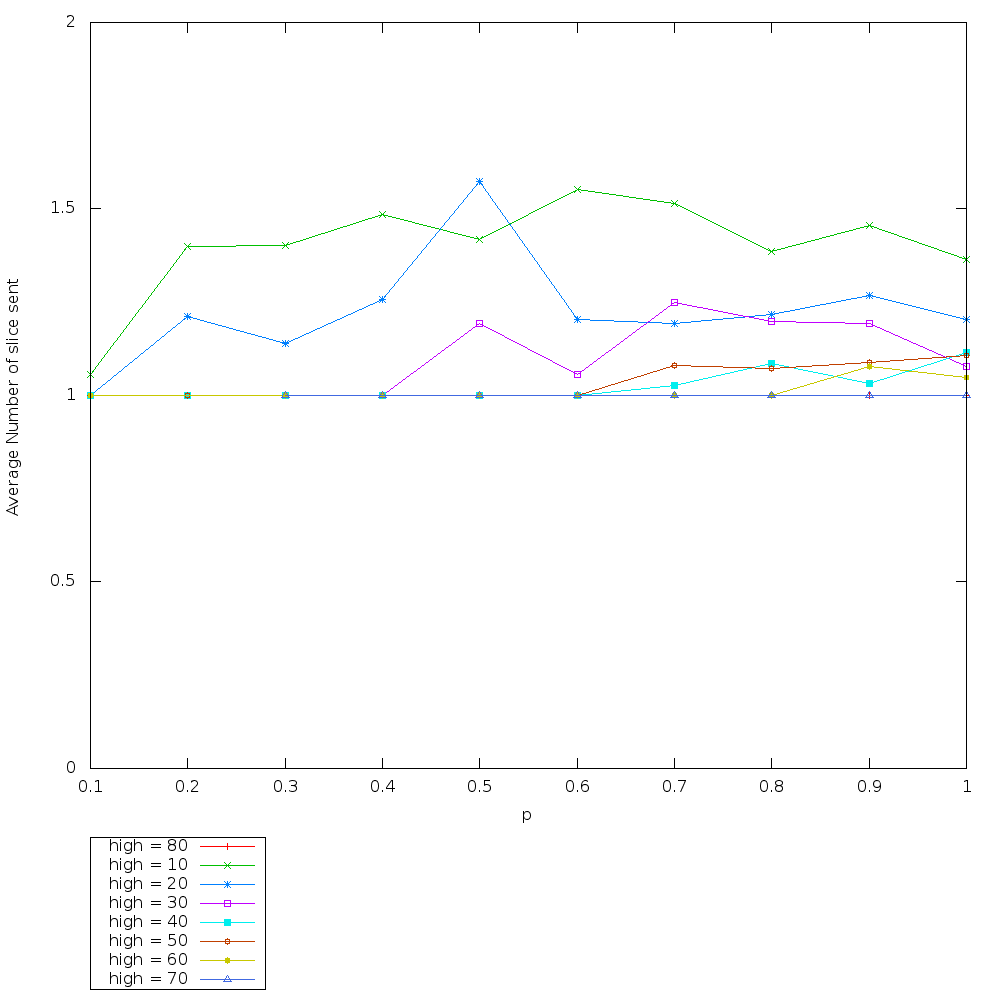
\includegraphics[height=10cm]{./image/slicesent/Nb_sent_slice.png}
  \caption{Graph of 1000 nodes with Slices of size 200}
 \end{figure}
 This graph underlines the fact that, whatever the shape of the DAG is, not a lot of slices are needed to synchronize. Therefore in this example the information sent by the client to synchronize fits in $20\times 320 \times 1.1 = 7040$ bits. $20$ is the number of hash functions we used, $320$ is the size of each table, and $1.1$ is the average number of slices.
 
 \paragraph{} The complexity of the \texttt{next\_ring} algorithm is difficult to assert, given that it mainly depends on the shape of the tree. However we counted the number of calls to the functions \texttt{pred} and \texttt{succ} as well as the number of visits to each nodes. We chose to count those calls because they are the one with the biggest complexity. The algorithm can be implemented without any call to the \texttt{succ} function, but the complexity of the algorithm is the same and it is more complicated to implement. The following curves show the average values of these calls divided by the size of the difference between the DAGs depending on different values. Each DAG had $1000$ nodes labelled with $160$ bits hash.
\begin{figure}[H]
 \centering
  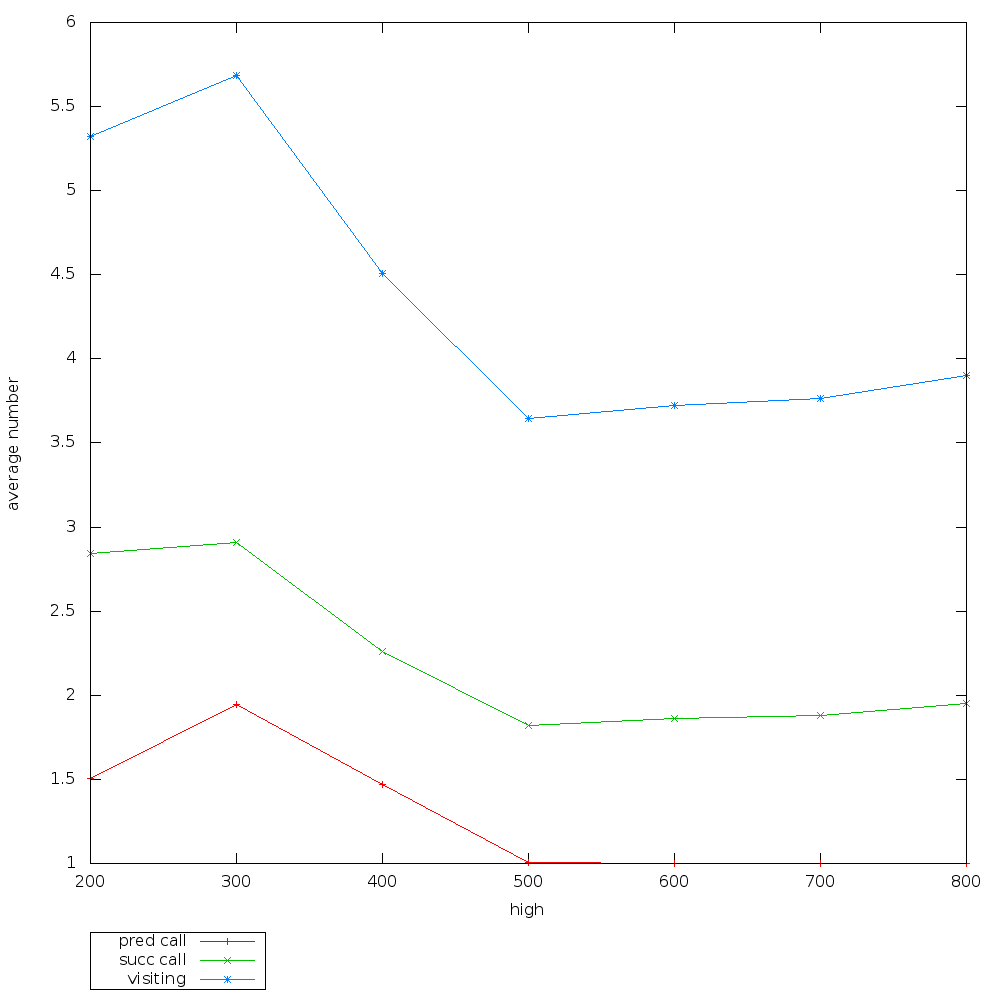
\includegraphics[height=10cm]{./image/eval/call_depending_on_high_over_size.png}
  \caption{Number of operations depending on the height of the DAG}
  \label{fig:3.6}
 \end{figure}
 \begin{figure}[H]
 \centering
  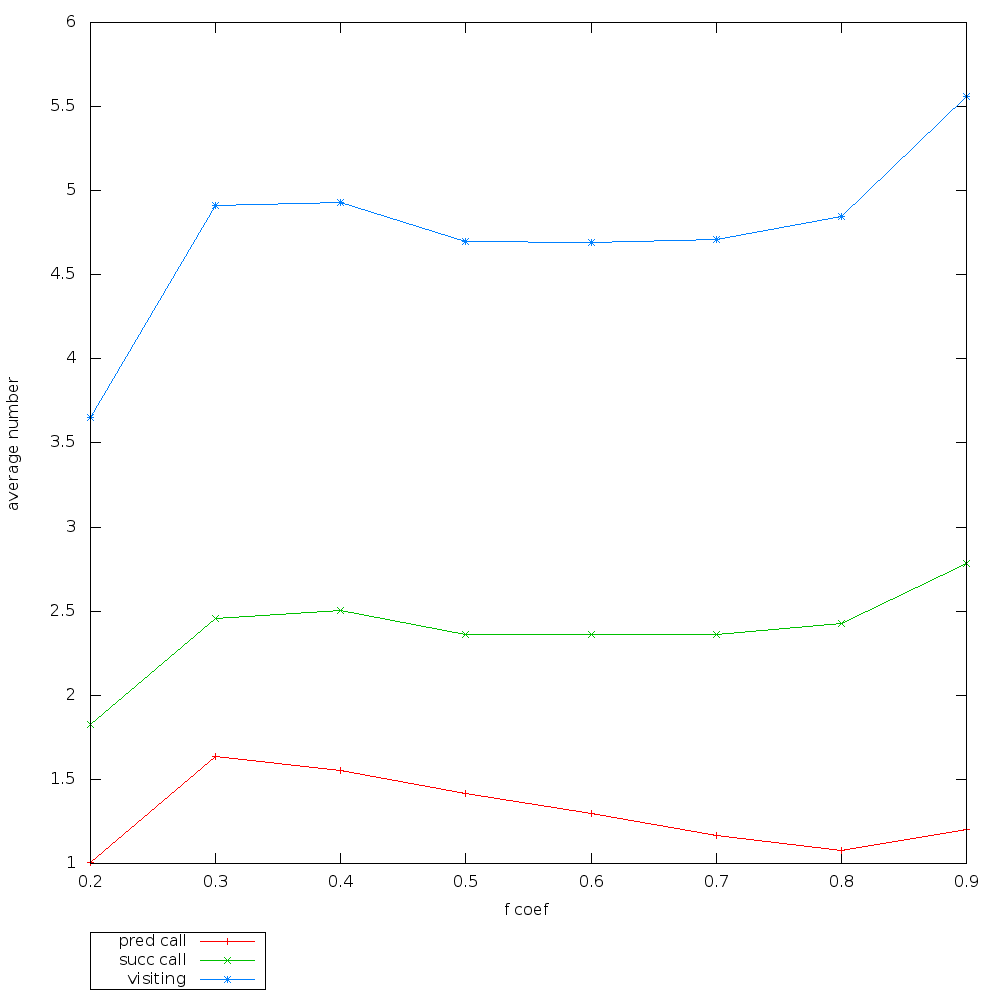
\includegraphics[height=10cm]{./image/eval/call_depending_on_f_coef.png}
  \caption{Number of operations depending on average number of predecessors}
 \label{fig:3.7}
 \end{figure}
 The two previous graphs (figure~\ref{fig:3.6} and figure~\ref{fig:3.7}) underline that the complexity in terms of call to the \texttt{pred} and \texttt{succ} function is linear in average on the size of the difference between the two DAGs that are being synchronized, which is the main result we wanted. Indeed in the case where we want our algorithm to work it is important that the complexity does not increase with the size of the history but only with the size of the difference.